\begin{chapter}{La détérioration visuelle suite au décodage de séquences vidéo H.264 corrompues}
\label{chap-erreur}
Jusqu'à présent, nous avons présenté la norme H.264 ainsi que les mécanismes lui
permettant de mieux résister aux pertes encourues lors de son transport sur des
réseaux peu fiables. L'approche typique adoptée pour réduire ces pertes est
d'augmenter la redondance. Cette dernière peut se manifester sous plusieurs
formes, tels l'encodage de trames redondantes ou la retransmission de paquets
manquants. Toutefois, cette redondance accroit le nombre de bits requis pour le
transport d'une séquence. Mais en pratique, pour plusieurs réseaux mobiles, la
bande passante est restreinte et, pour accommoder le nombre grandissant
d'utilisateurs ou pour respecter les délais \textit{temps réel}, ces mécanismes
ne peuvent pas être employés.

Dans ce chapitre, il sera question des notions reliées au décodage de séquences
H.264 corrompues et à la détérioration visuelle qui peut en résulter. À la
\sect{sect-decode}, nous expliquons l'impact de la corruption de bits sur
l'encodage entropique. Par la suite, la détérioration visuelle, issue du
décodage de trames \textit{inter} corrompues, est expliquée à la
\sect{sect-deterioration}. Finalement, nous présentons, à la
\sect{sect-propagation}, les différentes formes de propagations d'erreurs.

\begin{section}{Le décodage de paquets corrompus}
\label{sect-decode}
Vu la situation précédemment décrite, une solution intéressante pour la
résilience aux erreurs, qui n'augmente pas le fardeau des réseaux mobiles, est
d'améliorer l'efficacité de la dissimulation d'erreurs effectuée par le
décodeur. Le chapitre précédent fait mention des techniques de dissimulation
d'erreurs incorporées au décodeur inclus avec le
\ltCodec~\page{sect-dissimulation}. Ces techniques présupposent que l'ensemble
du paquet est corrompu. Ce nivèlement par le bas est partiellement dû à
l'architecture en couche utilisée pour l'interconnexion des systèmes, décrite
par \citet{Zimmermann1980} et présentée dans cet ouvrage, au
chapitre~\ref{chap-h264transport} \page{sect-RTP}. Cette architecture sépare,
dans deux couches distinctes, la réception des paquets et le décodage de leur
contenu. Ceci a plusieurs avantages, mais l'inconvénient majeur est de
restreindre l'interaction entre les couches. Par exemple, lorsque l'on détermine
au niveau d'UDP qu'un paquet est corrompu, ce dernier est rejeté. Ceci empêche
une application située aux couches supérieures, tel le décodeur H.264, d'avoir
accès aux paquets corrompus.

Le \textit{Joint source-channel decoding} \citep{Duhamel2010} est une approche
qui vise à établir une meilleure interaction entre les couches en combinant la
logique de la source (c.-à-d. la norme H.264) à l'analyse du contenu erroné d'un
paquet, afin de déterminer l'emplacement de l'erreur. Cette localisation de
l'erreur fait en sorte qu'au lieu de dissimuler l'ensemble du contenu du paquet,
la dissimulation serait effectuée seulement sur des codes contenant les bits
corrompus. Dans le cadre de la norme H.264, un algorithme de détection
d'erreurs d'une telle précision n'a pas encore été développé.

Une des raisons de la complexité de la détection d'erreurs dans des données
codées provient du fait que le codage cherche à éliminer la redondance. Cette
absence de redondance complexifie grandement la détection des erreurs.
Commençons par regarder le train de bits produit par un codage entropique à
taille variable, tels CAVLC ou Exp-Golomb. Dans ce genre de codage, une erreur
peut complètement changer le message, comme illustré à la \fig{fig-BitDesync}
(voir tableau~\ref{tab-ExpGolomb} pour les codes). Ceci est dû au fait
qu'altérer des bits change les codes et donc, leurs tailles et, par conséquent,
altère les codes subséquents jusqu'au prochain marqueur de synchronisation. Un
marqueur de synchronisation est une suite unique de bits servant à réinitialiser
la lecture de codes à taille variable.

\begin{figure}
	\fbox{ \centering
		\includegraphics{images/Bitstream.pdf}
	}
	\caption[Désynchronisation du train de bits]{Désynchronisation du train de
bits.\\ Adaptée de \citet[p.~11]{Ikuno2007}}
	\label{fig-BitDesync}
\end{figure}

\begin{table}
	\caption[Codes exponentiels Golomb]{Codes exponentiels Golomb. \\Adaptée de
\citet[p.~11]{Ikuno2007}}
	\vspace{-1em}
	\label{tab-ExpGolomb}
	\centering
  	\begin{tabular}{| c | c | }
    	\hline
    	\textbf{Code} & \textbf{Code Exp-Golomb}\\
    	\hline
    	0 & 1\\ \hline
    	1 & 010\\ \hline
    	2 & 011\\ \hline
    	3 & 00100\\ \hline
    	4 & 00101\\ \hline
    	5 & 00110\\ \hline
    	6 & 00111\\ \hline
    	7 & 0001000\\ \hline
    	8 & 0001001\\ \hline
  \end{tabular}
\end{table}


Cette désynchronisation peut mener à la désynchronisation du décodeur, voire
même, à faire planter\footnoteETS{Selon les auteurs, le terme plantage est
considéré comme usuel, familier ou appartenant à l'argot des informaticiens. Des
termes plus neutres, mais aussi plus généraux, comme incident et panne, ont été
proposés antérieurement ou sont encore parfois employés dans une langue plus
soutenue. Ils ne rendent toutefois pas l'idée première contenue dans
crash~\citep{GrandDic}.} ce dernier. D'une part, le décodeur plante suite à une
défaillance causée par la lecture de codes invalides. D'autre part, si le
décodeur ne plante pas, le décodage sera désynchronisé, c'est-à-dire que de
mauvais codes seront utilisés jusqu'au prochain marqueur de synchronisation.
Lorsque le décodeur reconstruit la trame avec ces mauvais codes, ceci peut
occasionner de la détérioration visuelle, comme celle présentée à la
\fig{fig-badImages}. C'est le cas à la \fig{fig-newsBad}, où la détérioration
visuelle n'est pas toujours évidente pour l'utilisateur.

\begin{figure}
	\fbox{\centering
		\minibox[c]{
			\subfloat[]{
				\includegraphics[width=0.42\linewidth]{images/akiyoBad.png}
				\label{fig-akiyoBad}}
			\subfloat[]{
				\includegraphics[width=0.42\linewidth]{images/carphoneBad.png}
				\label{fig-carphoneBad}}\\ %
			\subfloat[]{
				\includegraphics[width=0.42\linewidth]{images/foremanBad.png}
				\label{fig-foremanBad}}
			\subfloat[]{
				\includegraphics[width=0.42\linewidth]{images/newsBad.png}
				\label{fig-newsBad}}
		}
	}
	\caption[Détérioration visuelle issue d'un décodage désynchronisé] {Exemples de
la détérioration visuelle issue du décodage désynchronisé de paquets corrompus.}
	\label{fig-badImages}
\end{figure}

En ce qui concerne cette détérioration visuelle, elle est le sujet de la
prochaine section. Cependant, pour plus d'information sur la résilience du
décodeur, inclus dans le \ltCodec, face à la désynchronisation des codes
entropiques, veuilliez vous référer à la \sect{sec-ResilienceDecodeur}
<<\nameref{sec-ResilienceDecodeur}>> \page{sec-ResilienceDecodeur}.
\end{section}

\begin{section}{La détérioration visuelle}
\label{sect-deterioration}
Ici, notre analyse de la détérioration visuelle porte uniquement
sur celle issue du décodage de trames \textit{inter}, car c'est le type de
détérioration visuelle détectée par la solution proposée dans cet ouvrage. La
désynchronisation d'un bloc \textit{inter} peut survenir dans une ou
plusieurs de ces composantes : la trame de référence, le vecteur de mouvement ou
le résiduel.

D'une part, la détérioration visuelle engendrée par la corruption de la trame de
référence ou du vecteur de mouvement est très similaire, c'est-à-dire que le
contenu du bloc ne provient pas du bon endroit. Il provient soit de la mauvaise
trame de référence ou du mauvais emplacement dans la bonne trame. Cette
détérioration cause souvent des effets de bloc issus de la discontinuité
spatiale entre le contenu des bons blocs et celui du bloc erroné, comme illustré
à la \fig{fig-VectorsBad}.

\begin{figure}
	\fbox{\centering
		\minibox[c]{
			\subfloat[]{
				\includegraphics[width=0.88\linewidth]{images/VectorsBad3.png}
			\label{fig-VectorsBad3}}\\ %
			\subfloat[]{
				\includegraphics[width=0.42\linewidth]{images/VectorsBad1.png}
			\label{fig-VectorsBad1}}
			\subfloat[]{
				\includegraphics[width=0.42\linewidth]{images/VectorsBad2.png}
			\label{fig-VectorsBad2}}
		}
	}
	\caption[Détérioration visuelle issue de la corruption de la trame de référence
ou du vecteur de mouvement]{Exemples de la détérioration visuelle issue de la
corruption de la trame de référence ou du vecteur de mouvement.}
	\label{fig-VectorsBad}
\end{figure}

D'autre part, le résiduel corrompu produit un effet secondaire très différent de
celui issu la corruption de la trame de référence ou du vecteur de mouvement. Il
s'agit, ici, d'un bloc qui n'a pas l'apparence d'une image naturelle. Ceci est
dû à la corruption des indices transformés qui se produit dans le domaine de la
transformée. Le résultat de la transformée inverse des indices corrompus est un
bloc d'une seule couleur ou avec une texture non naturelle, comme c'est le cas à
la \fig{fig-ResBad}. Toutefois, cette détérioration produit souvent, elle aussi,
une discontinuité spatiale dans l'image.

\begin{figure}
	\fbox{\centering
		\subfloat[]{
			\includegraphics[width=0.25\linewidth]{images/ResBad1.png}
			\label{fig-ResBad1}} 
		\subfloat[]{
			\includegraphics[width=0.42\linewidth]{images/ResBad2.png}
			\label{fig-ResBad2}}
	}
	\caption[Détérioration visuelle issue de la corruption du résiduel]{Exemples de
la détérioration visuelle issue de la corruption du résiduel.}
	\label{fig-ResBad}
\end{figure}

\end{section}

\begin{section}{La propagation de la détérioration visuelle}
\label{sect-propagation}
Comme démontré à la \fig{fig-BitDesync} \page{fig-BitDesync}, une erreur
binaire peut avoir un impact considérable sur un train de bits, vu la
désynchronisation qu'elle engendre en ce qui a trait aux codes entropiques.
Néanmoins, cette erreur peut aussi avoir d'autres répercussions, si elle sert à
la prédiction d'autres blocs. Ce phénomène se nomme propagation d'erreurs. Il
peut survenir autant dans le domaine spatial que temporel.

Lorsque des pixels endommagés servent à la prédiction de trames subséquentes,
ceci permet à l'erreur de voyager d'une trame \textit{inter} à une autre. Il
s'agit, ici, d'une propagation temporelle de l'erreur. Cette propagation peut se
poursuivre jusqu'à la prochaine trame \textit{intra}. La \fig{fig-ErrorProp}
permet de visualiser la propagation d'erreurs dans le temps.

\begin{figure}
	\fbox{ \centering
		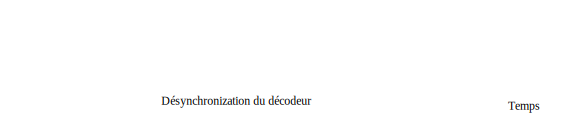
\includegraphics[width=0.97\linewidth]{images/ErrorPropagation.pdf}
	}
	\caption[Propagation temporelle de l'erreur] {Propagation temporelle de
l'erreur.\\ Adaptée de \citet[p.~1711]{Giro1999}}
	\label{fig-ErrorProp}
\end{figure}

La propagation spatiale d'erreurs peut survenir de deux façons, soit par les
vecteurs de mouvement ou par l'intermédiaire du filtre antiblocs. Les vecteurs
de mouvement sont sujets à la propagation d'erreurs, car ils sont prédits. Ce
qui fait en sorte qu'un vecteur de mouvement endommagé nuira aux autres vecteurs de
mouvement dont la prédiction repose sur celui-ci.

Le filtre antiblocs effectue, malgré lui, une propagation de l'erreur en bordure
des blocs lorsqu'il lisse ces dernières, afin d'en réduire les effets de bloc.
Le lissage d'une bordure d'un bloc corrompu propage la détérioration visuelle au
bloc voisin. Cette propagation est locale et ne s'étend pas plus loin que le
lissage, soit jusqu'à deux pixels à l'extérieur d'un bloc corrompu.
\end{section}

Dans ce chapitre, nous avons décrit la détérioration visuelle issue du décodage
de paquets corrompus. Typiquement, les paquets corrompus sont rejetés et ce
genre de détérioration ne se produit pas. Cependant, pour tirer profit du
contenu valide à l'intérieur de paquets corrompus, il faut décoder ces paquets
et donc faire face à cette détérioration. Pour ce faire, un nouveau type
d'algorithme a été développé, celui capable de détecter et de dissimuler la
détérioration visuelle. Avant de présenter l'algorithme
proposé~(chapitre~\ref{chap-mcb}), nous présentons d'abord ceux qui existent
déjà~(chapitre~\ref{chap-revuelit}).
\end{chapter}